% Template for PLoS

\documentclass[10pt]{article}

% amsmath package, useful for mathematical formulas
\usepackage{amsmath}
% amssymb package, useful for mathematical symbols
\usepackage{amssymb}

% hyperref package, useful for hyperlinks
\usepackage{hyperref}

% graphicx package, useful for including eps and pdf graphics
% include graphics with the command \includegraphics
\usepackage{graphicx}

% Sweave(-like)
\usepackage{fancyvrb}
\DefineVerbatimEnvironment{Sinput}{Verbatim}{fontshape=sl}
\DefineVerbatimEnvironment{Soutput}{Verbatim}{}
\DefineVerbatimEnvironment{Scode}{Verbatim}{fontshape=sl}
\newenvironment{Schunk}{}{}
\DefineVerbatimEnvironment{Code}{Verbatim}{}
\DefineVerbatimEnvironment{CodeInput}{Verbatim}{fontshape=sl}
\DefineVerbatimEnvironment{CodeOutput}{Verbatim}{}
\newenvironment{CodeChunk}{}{}

% cite package, to clean up citations in the main text. Do not remove.
\usepackage{cite}

\usepackage{color}

% Use doublespacing - comment out for single spacing
%\usepackage{setspace}
%\doublespacing


% Text layout
\topmargin 0.0cm
\oddsidemargin 0.5cm
\evensidemargin 0.5cm
\textwidth 16cm
\textheight 21cm

% Bold the 'Figure #' in the caption and separate it with a period
% Captions will be left justified
\usepackage[labelfont=bf,labelsep=period,justification=raggedright]{caption}

% Use the PLoS provided bibtex style
\bibliographystyle{plos}

% Remove brackets from numbering in List of References
\makeatletter
\renewcommand{\@biblabel}[1]{\quad#1.}
\makeatother


% Leave date blank
\date{}

\pagestyle{myheadings}
%% ** EDIT HERE **


%% ** EDIT HERE **
%% PLEASE INCLUDE ALL MACROS BELOW

%% END MACROS SECTION


\begin{document}

% Title must be 150 characters or less
\begin{flushleft}
{\Large
\textbf{Reproducible Research Demo: What Does This Code Do Again?}
}
% Insert Author names, affiliations and corresponding author email.
\\
  Ben Chan\textsuperscript{1*},
  Stephanie Renfro\textsuperscript{1},
  Thomas Meath\textsuperscript{1,2}\\
\bf{1} Center for Health Systems Effectiveness, Oregon Health \& Science University,  Portland,  Oregon,  USA
\\
\bf{2} Center to Improve Veteran Involvement in Care, Portland VA Medical System,  Portland,  OR,  USA
\\

\textasteriskcentered{} E-mail:   \href{mailto:chanb@ohsu.edu}{\nolinkurl{chanb@ohsu.edu}}
  
  

\end{flushleft}

\section*{Abstract}\label{abstract}
\addcontentsline{toc}{section}{Abstract}

Reproducible research is the idea that results are published along with
documentation of the coding steps that produced them. This additional
transparency fosters credibility and allows others to replicate the
findings and build upon them - and allows you to return to past work
with less head scratching! The need for reproducibility is only
increasing as datasets grow larger and data analyses become more
complex.

\section*{Author summary}\label{author-summary}
\addcontentsline{toc}{section}{Author summary}

The authors are all Research Associates at OHSU's Center for Health
Systems Effectiveness

\section*{Introduction}\label{introduction}
\addcontentsline{toc}{section}{Introduction}

This work was inspired by the following email from Farmer Ben.

\begin{quote}
From: Ben Chan\\Sent: Thursday, June 11, 2015 4:04 PM\\To: Stephanie
Renfro\\Subject: What to feed chicks

Hello,

I'm receiving 20 baby chicks next month. Can you help me decide what to
feed them? I'm choosing between the following four diets:

\begin{enumerate}
\def\labelenumi{\arabic{enumi}.}
\itemsep1pt\parskip0pt\parsep0pt
\item
  Grower diet\\
\item
  Layer diet
\item
  Breeder diet
\item
  High cluckage diet
\end{enumerate}

Thanks, Ben

\begin{center}\rule{0.5\linewidth}{\linethickness}\end{center}

Ben Chan, Farmer and Research Associate\\OHSU Center for Health Systems
Effectiveness\\Office: 3030 SW Moody \textbar{} Mail Code:
MDYCHSE\\www.ohsu.edu/chse
\end{quote}

\section*{Results}\label{results}
\addcontentsline{toc}{section}{Results}

Results and Discussion can be combined.

\subsection*{Preliminaries}\label{preliminaries}
\addcontentsline{toc}{subsection}{Preliminaries}

Start clock to calculate total runtime.

\begin{CodeChunk}
\begin{CodeInput}
start_program <- proc.time()
\end{CodeInput}
\end{CodeChunk}

Load needed packages:

\begin{itemize}
\itemsep1pt\parskip0pt\parsep0pt
\item
  \emph{data.table} - for faster processing\\
\item
  \emph{knitr} - for better tables (``kable'' function)
\item
  \emph{ggplot2} - for pretty plots\\
\item
  \emph{knitr} - for better table display
\end{itemize}

\begin{CodeChunk}
\begin{CodeInput}
packages <- c("data.table", "ggplot2", "knitr")
sapply(packages, require, character.only=TRUE, quietly=TRUE)
\end{CodeInput}
\begin{CodeOutput}
data.table    ggplot2      knitr 
      TRUE       TRUE       TRUE 
\end{CodeOutput}
\end{CodeChunk}

Define the CHSE color palette function.

\begin{CodeChunk}
\begin{CodeInput}
colorPalette <- function () {
  c(rgb(  1,  67, 134, maxColorValue=255),
    rgb(119, 120, 123, maxColorValue=255),
    rgb(139, 184, 234, maxColorValue=255),
    rgb(188, 190, 192, maxColorValue=255),
    rgb( 94, 122, 162, maxColorValue=255),
    rgb(223, 122,  28, maxColorValue=255))
}
\end{CodeInput}
\end{CodeChunk}

\subsection*{Prepare Data}\label{prepare-data}
\addcontentsline{toc}{subsection}{Prepare Data}

This demo uses
\href{http://www.inside-r.org/r-doc/datasets/ChickWeight}{data from an
experiment on the effect of diet on early growth of chicks},
\texttt{ChickWeight}, which comes pre-loaded in any R session.

Let's take a look at the first few rows:

\begin{CodeChunk}
\begin{CodeInput}
head(ChickWeight)
\end{CodeInput}
\begin{CodeOutput}
  weight Time Chick Diet
1     42    0     1    1
2     51    2     1    1
3     59    4     1    1
4     64    6     1    1
5     76    8     1    1
6     93   10     1    1
\end{CodeOutput}
\end{CodeChunk}

Let's also print a summary of the data.

\emph{Note, by specifying the option ``echo = FALSE'', the resulting
output will display, but not the code that generated it.}

\begin{CodeChunk}
\begin{CodeOutput}
     weight           Time           Chick     Diet   
 Min.   : 35.0   Min.   : 0.00   13     : 12   1:220  
 1st Qu.: 63.0   1st Qu.: 4.00   9      : 12   2:120  
 Median :103.0   Median :10.00   20     : 12   3:120  
 Mean   :121.8   Mean   :10.72   10     : 12   4:118  
 3rd Qu.:163.8   3rd Qu.:16.00   17     : 12          
 Max.   :373.0   Max.   :21.00   19     : 12          
                                 (Other):506          
\end{CodeOutput}
\end{CodeChunk}

Convert to data.table for faster processing.

\begin{CodeChunk}
\begin{CodeInput}
ChickWeight <- data.table(ChickWeight)
\end{CodeInput}
\end{CodeChunk}

Just for fun, let's create a table showing mean weight at times 0, 10,
and 21 days, for each of the four diet types.

\begin{CodeInput}
mean_ChickWeight <- ChickWeight[Time %in% c(0,10,21),
                                list(mean_weight = round(mean(weight), digits=1)),
                                by = list(Diet,Time)]

#kable(mean_ChickWeight)
\end{CodeInput}

Create a character variable for \texttt{diet}. Use this variable for
plotting small multiples.

\begin{CodeChunk}
\begin{CodeInput}
ChickWeight[, dietChr := sprintf("Diet %d", Diet)]
\end{CodeInput}
\begin{CodeOutput}
     weight Time Chick Diet dietChr
  1:     42    0     1    1  Diet 1
  2:     51    2     1    1  Diet 1
  3:     59    4     1    1  Diet 1
  4:     64    6     1    1  Diet 1
  5:     76    8     1    1  Diet 1
 ---                               
574:    175   14    50    4  Diet 4
575:    205   16    50    4  Diet 4
576:    234   18    50    4  Diet 4
577:    264   20    50    4  Diet 4
578:    264   21    50    4  Diet 4
\end{CodeOutput}
\end{CodeChunk}

\subsection*{Growth for Individual
Chicks}\label{growth-for-individual-chicks}
\addcontentsline{toc}{subsection}{Growth for Individual Chicks}

The following plot illustrates the growth curve for individual chicks
from 0 to 21 days.

Colors represent the four diets.

\textbf{From this plot, it is difficult to distinguish between the
performance of the four diets.}

\begin{CodeChunk}

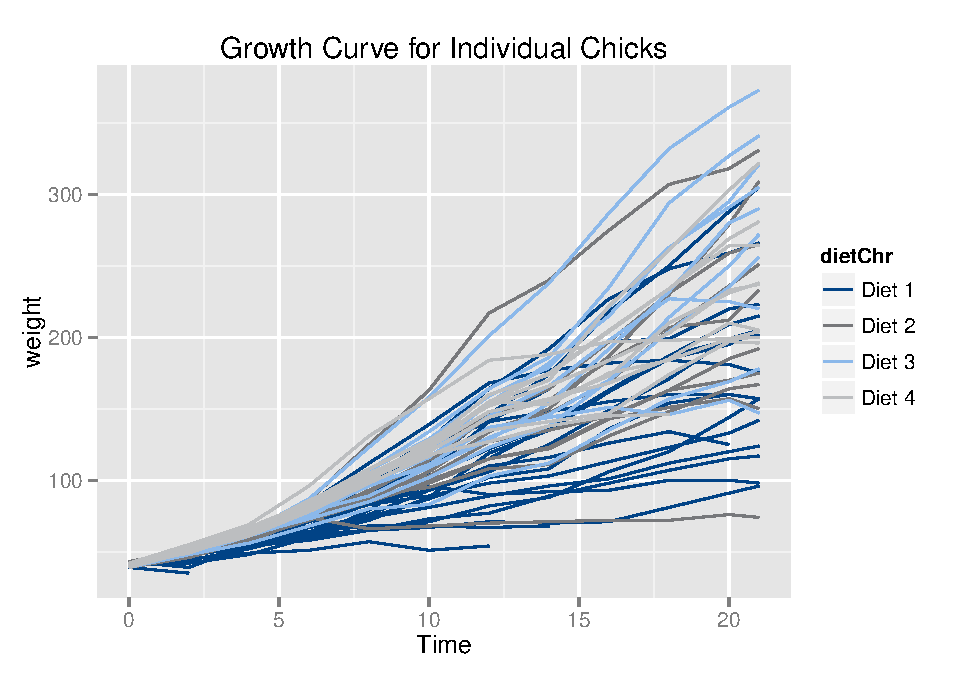
\includegraphics{ReproducibleResearchDemo_files/figure-latex/unnamed-chunk-9-1} \end{CodeChunk}

\textbf{Individual growth curves}

Plot individual chick growth curves using small multiples.

\begin{CodeChunk}

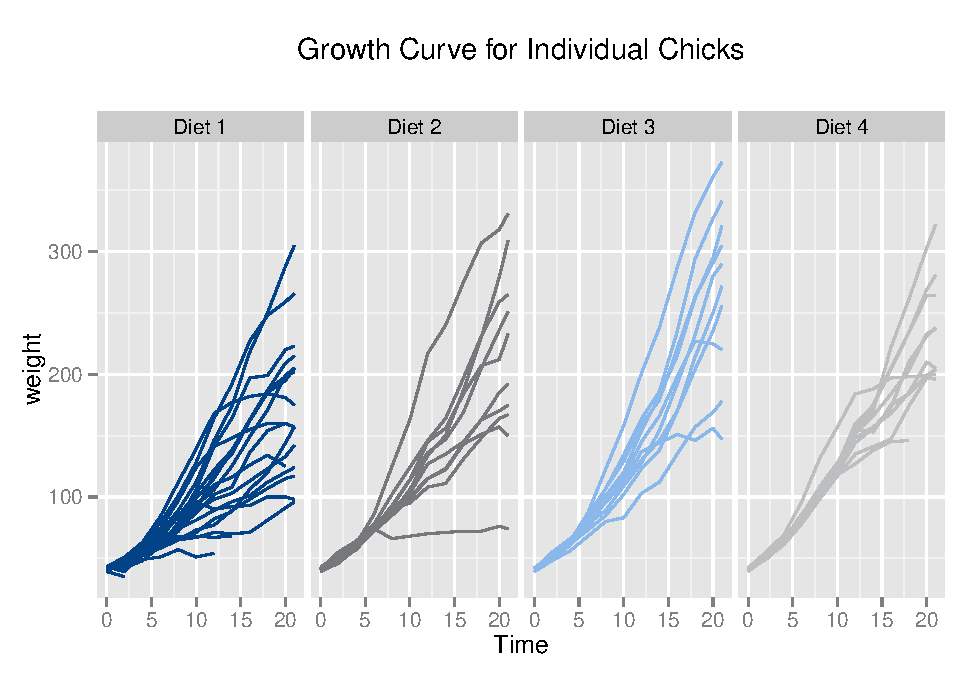
\includegraphics{ReproducibleResearchDemo_files/figure-latex/unnamed-chunk-10-1} \end{CodeChunk}

\textbf{Fitted growth curves}

Plot fitted growth curves using small multiples. Data points are
jittered around time value.

\begin{CodeChunk}

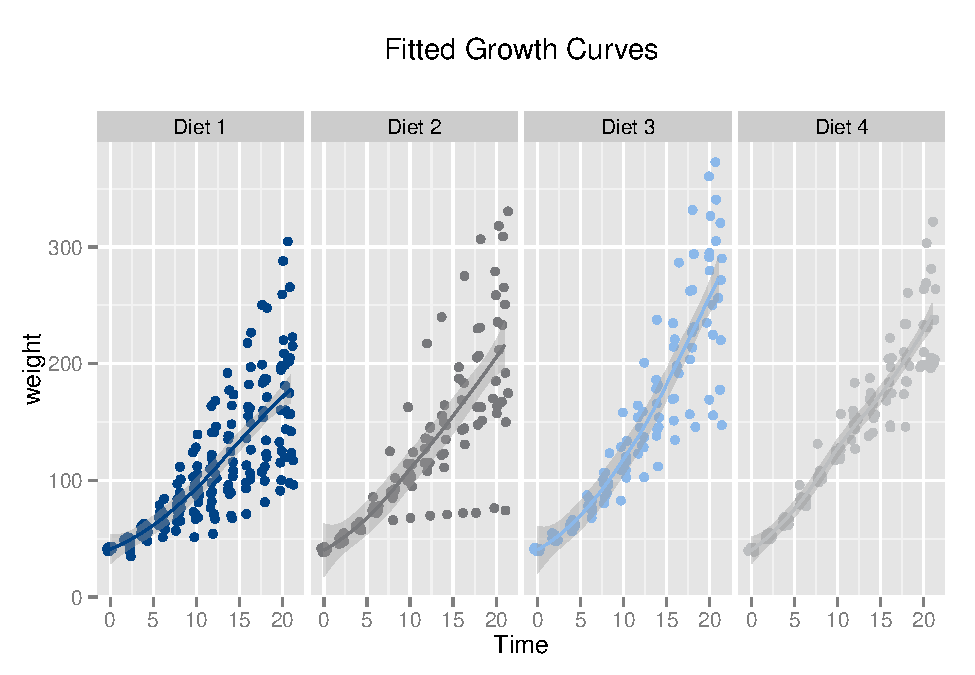
\includegraphics{ReproducibleResearchDemo_files/figure-latex/unnamed-chunk-11-1} \end{CodeChunk}

\textbf{Final weight density}

Plot densities by diet for chicks' final weights (day 21) using small
multiples.

\begin{CodeChunk}

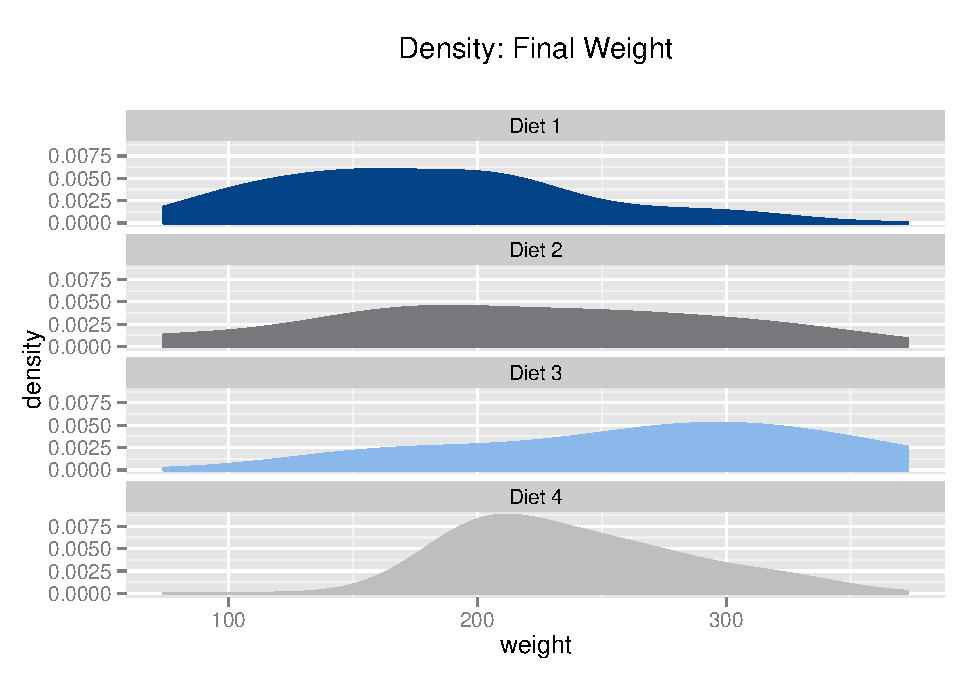
\includegraphics{ReproducibleResearchDemo_files/figure-latex/unnamed-chunk-12-1} \end{CodeChunk}

\subsection*{Wrap Up}\label{wrap-up}
\addcontentsline{toc}{subsection}{Wrap Up}

Calculate total runtime.

\begin{CodeChunk}
\begin{CodeInput}
time_program <- proc.time()-start_program
print(paste("Total runtime:", format(time_program[3]/60,digits=3), "minutes"))
\end{CodeInput}
\begin{CodeOutput}
[1] "Total runtime: 0.0852 minutes"
\end{CodeOutput}
\end{CodeChunk}

Clear memory.

\begin{CodeChunk}
\begin{CodeInput}
rm(list=ls())
invisible(gc())
\end{CodeInput}
\end{CodeChunk}

\section*{Discussion}\label{discussion}
\addcontentsline{toc}{section}{Discussion}

If this was a real paper, we would have some discussion about our
results. Because this is an example, we do not.

\section*{Methods}\label{methods}
\addcontentsline{toc}{section}{Methods}

This section is also not currently written out in full. This is where
your methods would go to satisfy PLOS.

\section*{Acknowledgments}\label{acknowledgments}
\addcontentsline{toc}{section}{Acknowledgments}

Rojo the Llama: for being a very friendly llama.

\section*{References}\label{references}
\addcontentsline{toc}{section}{References}

A reference list should be automatically created here. However it won't.
Pandoc will place the list of references at the end of the document
instead. There are no convenient solution for now to force Pandoc to do
otherwise. The easiest way to get around this problem is to edit the
LaTeX file created by Pandoc before compiling it again using the
traditional LaTeX commands.

\section*{Figure Legends}\label{figure-legends}
\addcontentsline{toc}{section}{Figure Legends}

Figure Legends would go in here

\section*{Tables}\label{tables}
\addcontentsline{toc}{section}{Tables}

Tables would go here:

\end{document}

